\chapter{Kalibrering}
\label{cha:kalibrering}

For at kunne oversætte mellem udstyrets kanalnummer og en given energi skulle der foretages en
kalibrering. Til dette formål blev der benyttet en kilde, der bestod af tre $\alpha$-kilder:
\ce{^{241}Am}, \ce{^{239}Pu} og \ce{^{244}Cm}.

Idet forstærkningen er indstillet forskelligt i de enkelte strips og sektorer, er det
nødvendigt at kalibrere dem enkeltvis. Linierne er skarpt adskilte, derfor kan kalibreringen udføres
ved at fitte lineært til deres centroid værdier.  

Det skulle dog vise sig ikke at være helt så nemt, idet detektoren havde et inativt område, der blot
bremsede partiklen uden at registre energien. Dette dødlag havde en tykkelse $\Delta x$ på et par
mikrometer. Dette er illustreret på \ref{fig:deadLayer}.

Det medfører, at partikler, der rammer længere ude på detektoren, vil miste mere energi end de,
der rammer de inderste strips. De relevante størrelser er den målte energi $E_{0}$, energien før
dødlaget $E$ og vinklen $\phi$ mellem partiklens hastighed og detektorens normal. Ud fra nogle enkelte
geometriske betragtninger kan et udtryk for $E$ opskrives
\begin{equation}
  \label{eq:deadE}
  E = E_{0} + \d{E}{x} \frac{\Delta x}{\cos \phi}  .
\end{equation}
Det sidste led er energitabet i dødlaget, som afhænger af stoppeevnen, $\d{E}{x}$, af
materialet. Denne antages konstant gennem dødlaget. 
\begin{figure}[h]
  \centering
  \includegraphics[width=7cm]{DeadLayer}
  \caption{Skematisk tegning af S3 dektoren med et dødlag.}
  \label{fig:deadLayer}
\end{figure}

\section{Estimation af dødlagets tykkelse}
\label{sec:dodlag}

For at kunne bestemme tykkelsen af dødlaget er det nødvendigt at kende energien ved forskellige
vinkler, men som sagt er forstærkningen indstillet forskelligt i ringene.

% Løsningen på dette er at udvælge en radial sektor. Hver gang denne sektor bliver ramt, findes de
% cirkulære strips, hvor kanalnummeret er det samme plus minus et vist offset. Offsettet korrigerer
% for at forstærkningen ikke er den samme. Kanalnummeret fra de radiale sektor tilføjes så til et
% histogram for den cirkulære strip, der matchede. På denne måde er det muligt, at bestemme spektret
% for de enkelte cirkulære strips, udtrykt i den radiale sektors kanalnummer.

Løsningen på dette er at udvælge en radial sektor. Hver gang denne sektor bliver ramt, så matches
den med de cirkulære strips, der er ramt. Kriteriet for match er, at deres kanalnumre stemmer
overens inden for et vidst offset. Dermed er det muligt at bestemme spektret for de enkelte
cirkulære strips udtrykt i kanalnummeret for den radiale sektor.

I alle disse spektre bestemmes så centroidværdien af \Pu toppen, og kanalnummeret af denne.
Kanalnumrerne blev normaliseret til kanalnummeret i strip 1 og blev plottet som funktion af
$1/{\cos \phi}$. Ud over dette er \cref{eq:deadE}, for forskellige tykkelser, også plottet. Disse er
normaliseret til det teoretiske udtryk for strip 1. Stoppeevnen er taget fra \cite{Ziegler}.

Det er ikke muligt at lave et fit til data med $\Delta x$ som en fri parameter, så derfor er tykkelsen af
dødlaget vurderet ud fra de teoretiske kurver, som er plottet på \cref{fig:dead}. Data er
konstistent med en tykkelse på hhv. \SI{3.3(5)}{\um} og \SI{4.2(5)}{\um} for upstream- og
downstreamdektoreren.

\begin{figure}[h]
  \centering
  \subtop[Upstream]{\includegraphics[width=0.47\columnwidth]{DeadLayerThin}}%
  \hfill
  \subtop[Downstream]{\includegraphics[width=0.47\columnwidth]{DeadLayerThick}}%
  \caption{De normaliserede energier som funktion af $1/{\cos\phi}$. Kurverne angiver det teoretiske
    udtryk givet i \cref{eq:deadE} og er plottet for forskellige tykkelser.}
  \label{fig:dead}
\end{figure}


\section{Kalibreringsalgoritmen}
\label{sec:kalalgo}
\fxnote{Overvej denne overskrift}

Når tykkelsen er kendt, kan den målte energi $E_{0}$ bestemmes. Dermed kan vores detektorer
kalibreres. Fordi energitabet både afhænger af indgangsenergien og hvilken partikel, der er tale om,
så er det nødvendigt, under databehandlingen, at bestemme energitabet for hver enkel hændelse.

For energier hvor stoppeevnen er stor, så vil det give anledning til en fejl, hvis energitabet anses
som konstant hele vejen igennem materialet. Det samlede tab skulle istedet udregnes som et
integral. Istedet benyttes projected range, som er middel rækkevidden af en partikel i et givent
materiale, og ækvivalent til \cref{eq:deadE} kan den samlede rækkevidde skrives som
\begin{equation}
  \label{eq:deadR}
  R(E) = R(E_{0}) + \frac{\Delta x}{\cos \phi} .
\end{equation}

For at bestemme energien af en given hændelse, så bestemmes først den samlede rækkevidde, hvor
$R(E_{0})$ bestemmes ved tabelopslag. Dernæst regnes baglæns hvormed energien bestemmes ud fra
rækkevidden. 











